\section{Process Perspective}

\subsection{CI/CD Chain}

To introduce continuous integration and continuous deployment to the program, we used GitHub Actions. The project included several different workflows like provision and deploy as described in Table \ref{tab:workflows}.

\begin{table}[H]
    \centering
    \begin{tabular}{|p{0.4\textwidth} | p{0.55\textwidth}|}
        \hline
        \textbf{Workflow file} & \textbf{Function}\\
        \hline
        \textit{AutomaticBuildRelease.Backend} &  Bumps the patch versioning of the \textit{MinitwitSimulatorAPI} project and creates a release on the GitHub repository.\\
        \textit{AutomaticBuildRelease.Frontend} & Bumps the patch versioning of the \textit{Minitwit} project and creates a release on the GitHub repository.\\
        \textit{WeeklyMinorRelease} & Bumps the minor version of the entire program and creates a release each Thursday at 20:00 UTC.\\
        \textit{Linters-and-Formatter} & Runs Hadolint, Pre-commit, and the dotnet-format linter, when a PR is created, modified, and reopened.\\
        \textit{Testing} & Runs all tests on the infrastructure, the frontend, and the backend, when a PR is created, modified, and reopened.\\
        \textit{Provision-and-Deploy} & Provision and deploy swarm and observability servers using Ansible for server provision and Pulumi for infrastructure as code, on pushes to main.\\
        \textit{latex-build} & Creates a report PDF when changes have been made to the report.\\
        \hline
    \end{tabular}
    \caption{The function of the workflows}
    \label{tab:workflows}
\end{table}

Figure \ref{fig:workflows} visualises the development pipeline all the way from writing code to production. This includes running pre-commit to check for formatting, to passing both UI and integration tests as well as building and deploying.

\begin{figure}[H]
    \centering
    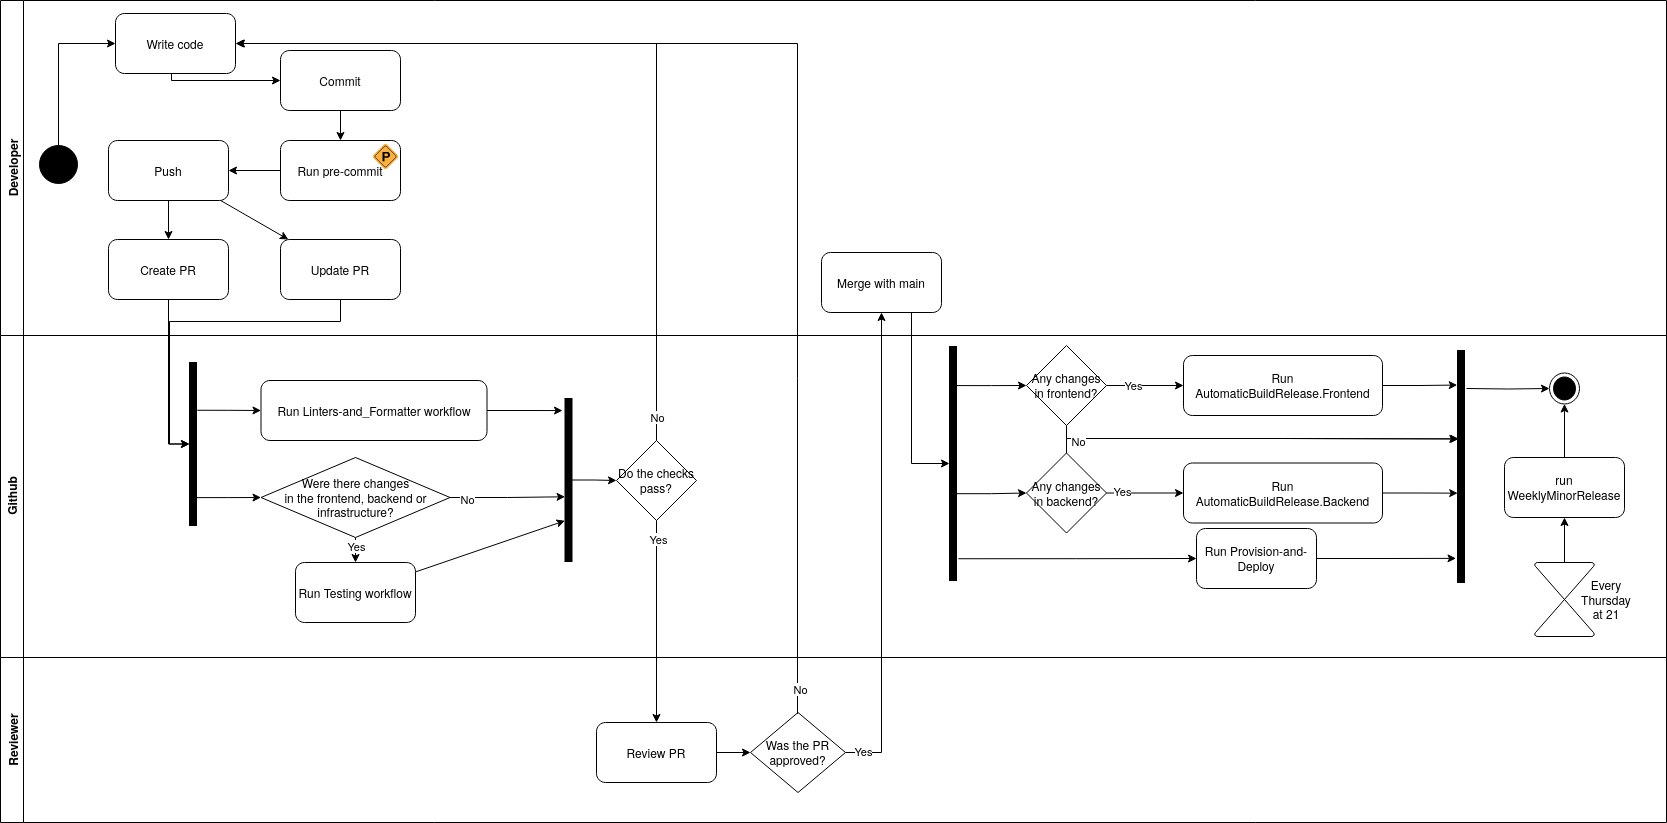
\includegraphics[angle=270, scale=0.37]{Github-Actions.png}
    \caption{Activity diagram showcasing the workflows interacting }
    \label{fig:workflows}
\end{figure}

\subsection{Monitoring and Logging}
For monitoring we use Grafana. We export metrics using OpenTelemetry, collect the metrics via Prometheus, and lastly push them to Grafana. Our board shows requests duration, errors rate, top 10 unhandled exception endpoints and more (for visualisation of the board, see appendix \ref{appendix:grafana}). We have used the board to get an overview of where to put our focus, ie. which endpoints to improve, which errors to fix, etc. Moreover, we have gained insights into the health of the system and an impression of how the backend and frontend handle requests.

For logging, we use Grafana and Loki. The logs are divided into Information, Warning, Debug and Error. All logging statements are placed in the controllers, such that we have information about the users' whereabouts in the system.

\subsection{Security Assessment}
Based on our security assessment (see appendix \ref{appendix:securityassesment}), we constructed the following risk matrix:
\begin{figure}[H]
    \centering
    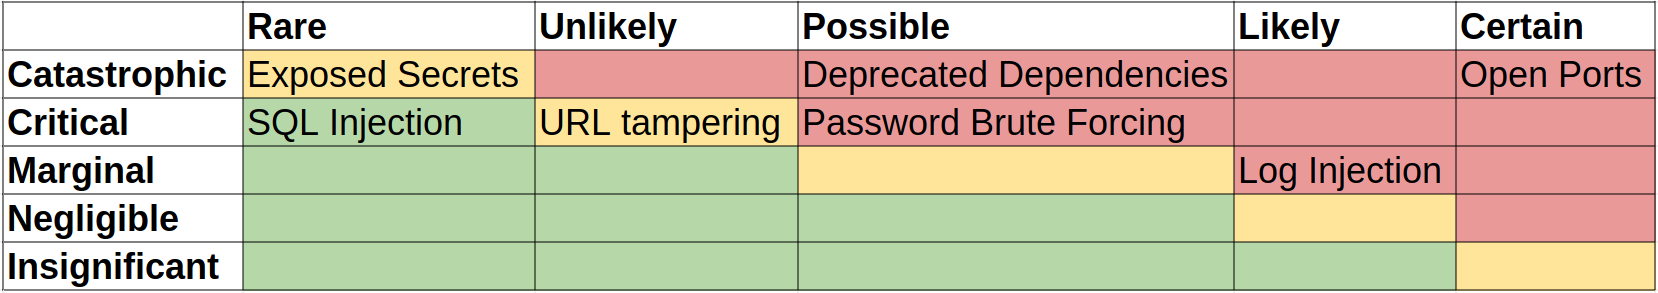
\includegraphics[width=1\linewidth]{images/risk-matrix.png}
    \caption{Risk matrix from security assessment}
    \label{fig:enter-label}
\end{figure}
We decided to focus on the scenarios in the red zone, as they would cause the most damage. Due to the team not having enough knowledge about how the simulator worked in regards to login and passwords, we did not move further with the \textit{Password Brute Forcing} scenario. However, possible solutions for a system in production include incorporating 2FA and password requirements.

For \textit{Log Injection}, we sanitised user inputs, as they previously were put directly into the log, which could be exploited by using injection attacks to hide ill-intentioned actions.

With \textit{Deprecated Dependencies}, we integrated the tool Dependabot into our CI/CD pipeline to identify outdated dependencies in our main repository. This ensures that an adversary is not able to take advantage of vulnerabilities in used tools.

\textit{Open Ports} was deemed the biggest risk, as this was presumably the reason we were hacked, which we have written about in further detail in section \ref{section_hacked}. We used the tool \texttt{nmap} to scan the IP address of our application and check for open ports, which showed the following:
\begin{figure}[H]
    \centering
    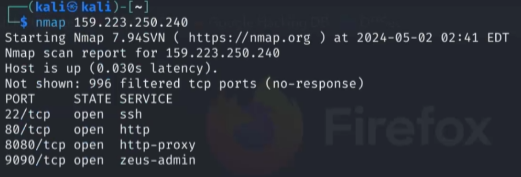
\includegraphics[width=1\linewidth]{images/nmap.png}
    \caption{Open ports found by nmap}
    \label{fig:matrix}
\end{figure}
We tried to close port 9090, which was used for Prometheus, but it was unclear if we succeeded as \texttt{nmap} and the firewall configurations contradicted each other. This was likely caused by Docker bypassing our firewall, which was handled by the Ansible \texttt{ufw} module, through IP tables.

\subsection{Scaling}
We use horizontal scaling, as we wanted a more resilient application and limit downtime when deploying. We settled on Docker Swarm over building a custom load balancer or adopting Kubernetes, due to its simplicity and compatibility with the existing system setup. To implement Docker Swarm we created a new server in our system and added a manager and a worker node to the Swarm.

When attempting to scale by adding another frontend replica, we encountered challenges. In order for the two replicas to work together, we needed to handle distributed sessions to remember who is logged in, even though the frontend replica is switched. However, we did not succeed in this (week 11 in appendix \ref{appendix_log}), which is why we only have a single frontend replica.

For the update strategy we went with rolling updates as it is the default option for Docker Swarm.
